
 \newpage
\subsection{SPI Interface}
This section describes the protocol used to communicate with the chip.

As an attempt to save time on implementation, the group decided to deviate from the standard SPI protocol and create an specialized protocol for the chip.
The total amount of data that should be sent, during each active period of the SPI enable, is 4x4 16-bit words to the chip and four 17-bit words from the chip. This is illustrated in Fig. \ref{spi_data} where the 4x4 16-bit words are grouped into four 64-bit words.

\begin{figure}[H]
\centering
\captionsetup{justification=centering}
\includegraphics[scale=0.2]{../figures/spi_data.png}
\caption{SPI data diagram}
\label{spi_data}
\end{figure}

The chip receive and send data with the most significant bit first. The order of the bits is illustrated Fig. \ref{spi_int}. Data is both written and read by the chip on the rising edge of the the SPI clock. This means that the circuitry communicating with the chip has to read and write on the falling edge of the clock. The first input data should be available on the first rising edge after SPI enable goes low, and the first bit of the output will be available on the first falling edge after SPI enable goes low. This can also be seen in Fig. \ref{spi_int}.\\

\begin{figure}[H]
\centering
\captionsetup{justification=centering}
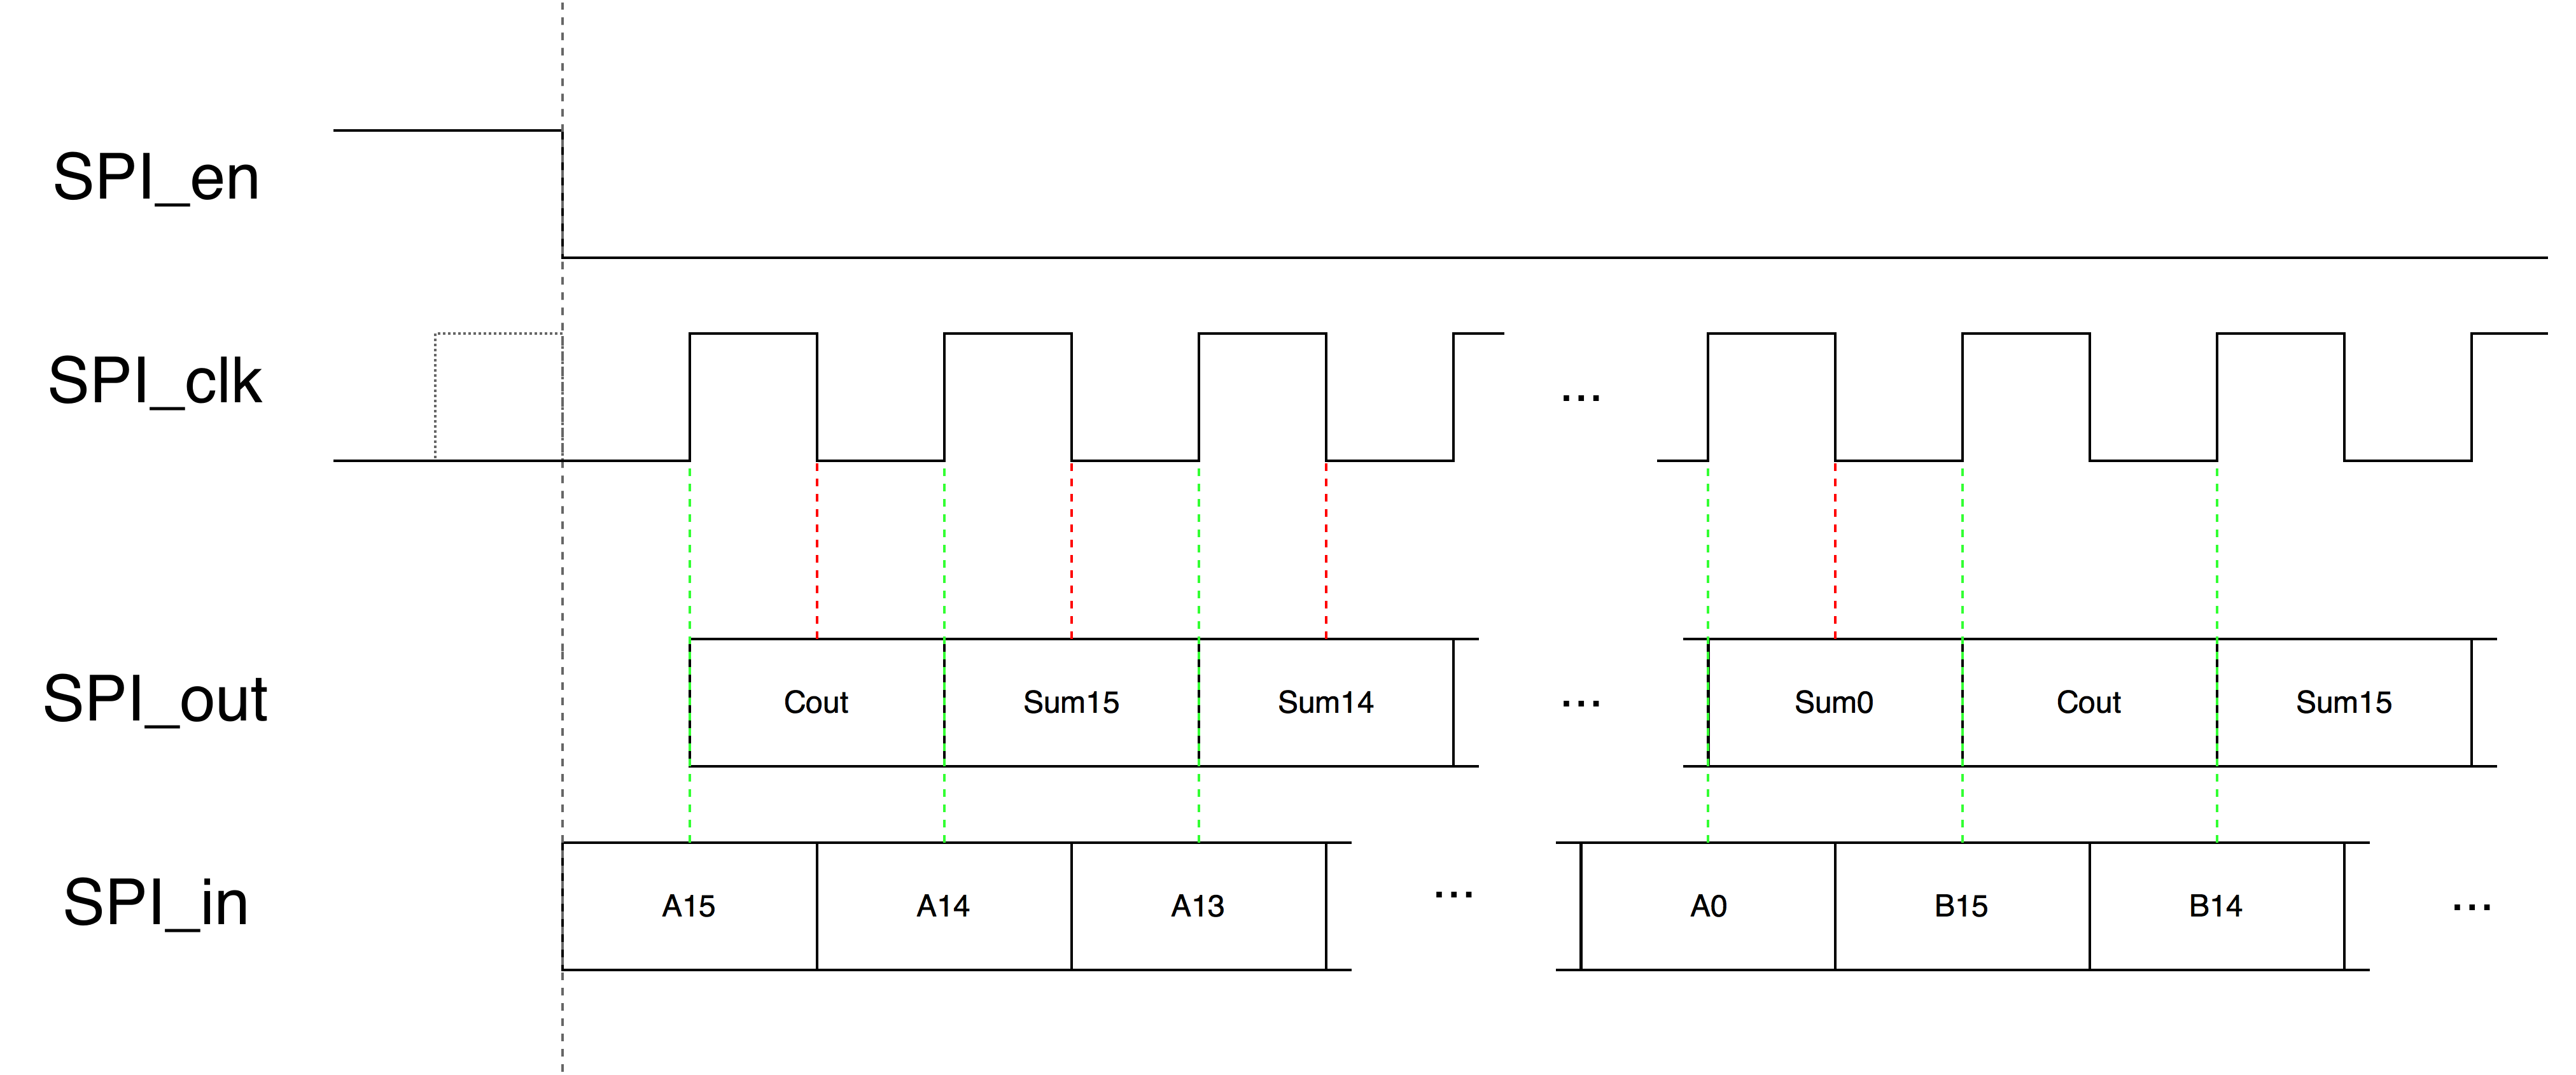
\includegraphics[scale=0.1]{../figures/spi_interface.png}
\caption{SPI timing diagram}
\label{spi_int}
\end{figure} 


Worth mentioning is that the SPI clock should be kept low while SPI enable is high. This can also be seen in Fig. \ref{spi_int} but might not be as clear.

